\subsection{Bibliothèque \texttt{\gls{game_logic}}}

Dans le chapitre \ref{subsection_architecture_generale} nous avions introduit le module conceptuelle \og Rule Book \fg{}, qui génère un ensemble de pairs coup possible et plateau conséquence. Pour ce faire ce module doit pouvoir décider de la légalité d'un coup et de connaître ses conséquences. 

Nous avions également parlé dans le chapitre \ref{section_analyse_environnement} d'un agent \og Arbitre \fg{} maître du jeu qui a besoin d'un ensemble de règles à fin d'initialiser le plateau et d'appliquer ou de refuser les coups respectivement légaux et illégaux.

Il est claire que ces deux objets partagent un même ensemble de fonctions et de structures, donc une bibliothèque que nous appèlerons \texttt{game\_logic}  :

\begin{figure}[H] 
\centering
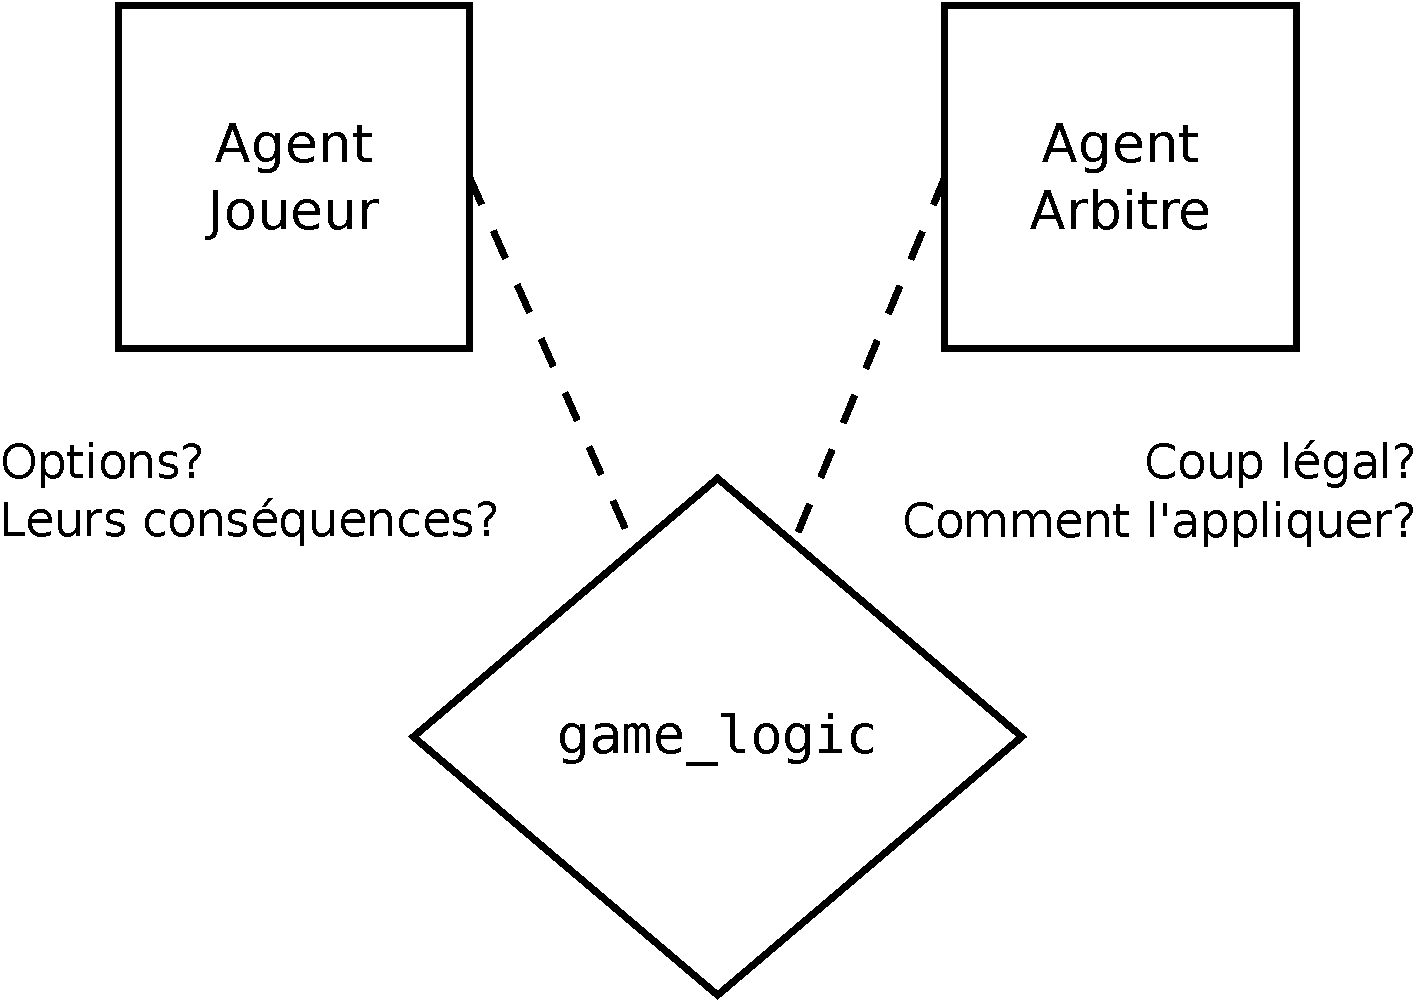
\includegraphics[width=\textwidth]{files/env/game_logic_shared} 
\caption{Partage de la bibliothèque \texttt{game\_logic}} 
\label{game_logic_shared}
\end{figure}

Précisement cette bibliothèque contient trois classes principales :

\begin{itemize}
\item \texttt{BoardMatrix} : Plateau sous forme matricielle avec accesseurs adaptés.
\item \texttt{Rules} : Interface implémenté par chaque jeu. Ses méthodes permettent de connaître :

\begin{itemize}
\item La forme du plateau et sa configuration initiale.
\item Qui joue en premier.
\item Quand la partie est gagné ou perdu et par qui, quand le match est nul.
\item Les coups possibles pour un joueur donnée.
\end{itemize}

\item \texttt{Game} : Associe un \texttt{Rules}, un \texttt{BoardMatrix}, un état et un joueur courant.
\end{itemize}

\begin{figure}[H] 
\centering
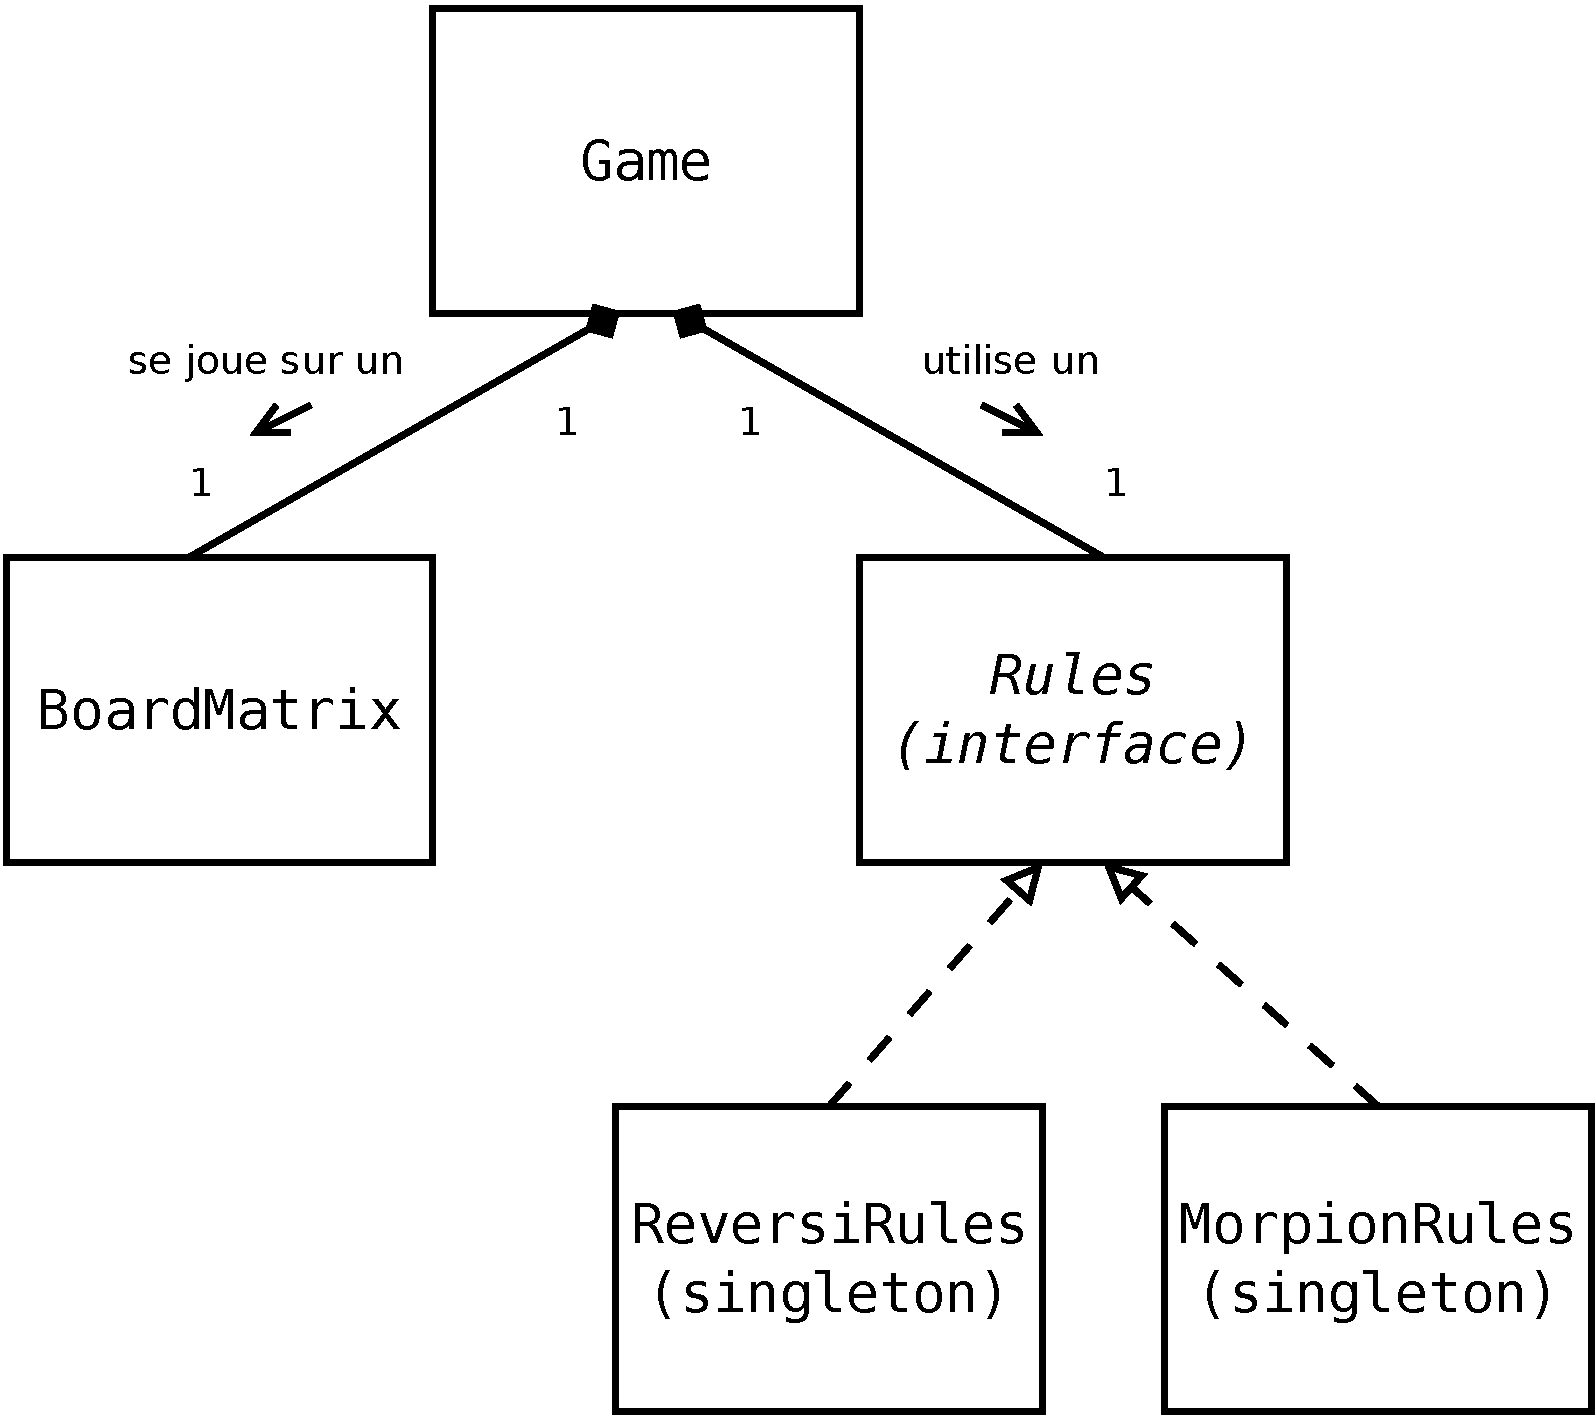
\includegraphics[width=\textwidth]{files/env/game_logic} 
\caption{Classes de la bibliothèque \texttt{game\_logic}} 
\label{game_logic}
\end{figure}


\subsection{Serveur \texttt{game\_service}}

Le chapitre \ref{section_analyse_environnement} conclut en proposant le modèle client-serveur pour les communications entre l'\emph{agent-joueur} et l'\emph{agent-arbitre}. L'arbitre et l'environnement, c'est à dire l'état du jeu, seront hébergés dans une application à part entière: un \og web service \fg{} appelé \texttt{game\_service}.
 
\subsubsection{\og Representational State Transfer \fg{} }

Le client-joueur a tout d'abord besoin de connaître l'état du jeu. Pour simplicité nous ne ferons aucun authentification ou de suivi du client, donc des requêtes \texttt{GET} de l'\texttt{HTTP}\footnote{ HTTP : Hyper-text transfer protocol. } nous suffirons. Ce protocole pilier du web il a l'avantage d'être très répandu, et cet ubiquité assure l'existence de documentation et de  bibliothèques ouvertes, complètes et simples d'utilisation pour tout langage et plateforme. 
Étant donnée que le développement du serveur ait débuté bien avant le reste du système ce choix nous permettait d'éviter d'avoir trop de contraintes par la suite.

\subsubsection{ Paramétrage de l'URL }

Le client a aussi besoin d'envoyer des coups au serveur. Pour ceci il suffit d'utiliser les paramètres de l'URL pour indiquer qui nous sommes et où nous jouons. De cette manière il est possible de préciser en plus 
\begin{itemize}
\item le joueur qui fait le coup,
\item le jeu
\item une ligne et une colonne,
\end{itemize}
Il est donc possible de joueur dans un browser en écrivant à la main les requêtes.

\subsubsection{Servlets Java}
Plus précisément la technologie Java Servlet est utilisé pour implémenter le gestionnaire de jeux. Un Servlet est une classe Java instancié par un serveur telle Tomcat ou Glassfish pour répondre à une requête HTTP spécifique. L'objet est détruit immédiatement après avoir envoyé sa réponse, généralement sous forme de string HTML ou XML.
Solution peu puissance et surtout peu intuitive pour les concepteurs web non-programmeurs, elle est le plus souvent utilisé pour le prototypage de sites web dynamiques avant de passer à une technologie plus complet comme JSP ou PHP. Cependant pour notre application il suffit très largement.